\section{Experiments}
\label{sec:experiment}

To comprehensively evaluate \method{} as a semantic search framework for factor discovery, we address three research questions:
\begin{enumerate}[leftmargin=*,itemsep=1pt,topsep=2pt]
    \item[\textbf{RQ1}:] Does schema-guided semantic search improve the quality of the discovered factor pool over representative alpha mining baselines?
    \item[\textbf{RQ2}:] Which components of \method{} contribute to its effectiveness?
    \item[\textbf{RQ3}:] Is the framework robust across schema-to-code backends, and can the learned scorer identify promising semantic regions before implementation?
\end{enumerate}
\subsection{Experimental Setup}

\paragraph{Dataset and Metrics.}
Following recent Qlib-based alpha-mining studies, we use the CSI300 universe as the primary benchmark. The time span is split into training (Jan 1, 2016 -- Dec 31, 2020), validation (Jan 1, 2021 -- Dec 31, 2022), and testing (Jan 1, 2023 -- Dec 31, 2025). The prediction target is the 5-day forward close-to-close return computed from daily OHLCV-style market data. We report factor predictive metrics (IC, ICIR, RankIC, RankICIR) and strategy metrics based on benchmark-relative excess returns (AER, IR, MDD). Data-processing, trading-cost, and metric definitions are provided in Appendix~\ref{sec:appendix_eval_details}.



\paragraph{Baselines.}
We compare against four families of baselines. \emph{Machine-learning predictors} include MLP and XGBoost \cite{chen2016xgboost}. \emph{Deep sequence models} include Transformer \cite{vaswani2017attention}, GRU \cite{cho2014learning}, and LSTM \cite{hochreiter1997long}. \emph{Open-source factor libraries} include Alpha158 and Alpha360 \cite{yang2020qlib}. \emph{Agentic mining systems} include RD-Agent \cite{li2025rdagentquant}, QuantaAlpha \cite{han2026quantaalpha}, and AlphaPROBE \cite{guo2026alphaprobe}. For reproduced agentic mining runs and \method{}, the LLM backend is fixed to the GPT-5.4 API under matched call and candidate-evaluation budgets. Predictor baselines are trained directly under the same train/validation/test split. Since the compared baselines do not support controlled fundamental-schema mining, we report both an OHLCV-only version of \method{} for the fair comparison and a +Fundamental version to show the additional schema modality supported by our framework.


\subsection{Main Results}

\subsubsection{Pool-Level Evaluation}

\begin{table*}[t]
\centering
\caption{Main-result table on CSI300. ``Fund. Schema'' indicates whether the mining process is allowed to use fundamental semantic schema fields. Higher is better for all metrics except MDD. Best results are bolded and second-best results are underlined; the pending AlphaPROBE reproduced run is excluded from ranking.}
\label{tab:main_eval}
\setlength\tabcolsep{3.0pt}
\small
\resizebox{0.98\textwidth}{!}{
\begin{tabular}{llcccccccc}
\toprule
\multirow{2}{*}{\textbf{Category}} & \multirow{2}{*}{\textbf{Method}} &
\multirow{2}{*}{\makecell{\textbf{Fund.}\\\textbf{Schema}}} &
\multicolumn{4}{c}{\textbf{Factor Predictive Power}} &
\multicolumn{3}{c}{\textbf{Strategy Performance}} \\
\cmidrule(lr){4-7}\cmidrule(lr){8-10}
 & & &
\textbf{IC} & \textbf{ICIR} & \textbf{Rank IC} & \textbf{Rank ICIR} &
\textbf{IR} & \textbf{AER (\%)} & \textbf{MDD (\%)$\downarrow$} \\
\midrule
\rowcolor[RGB]{242,244,247}\multicolumn{10}{c}{\textit{\textbf{Machine-Learning Predictors}}} \\
\multirow{2}{*}{\makecell[l]{Machine\\Learning}}
& MLP & \xmark & 0.0236 & 0.1408 & 0.0389 & 0.2471 & 0.5901 & 5.16 & 11.47 \\
& XGBoost & \xmark & 0.0284 & 0.2024 & 0.0373 & 0.2699 & 0.3556 & 2.55 & \second{10.30} \\
\midrule
\rowcolor[RGB]{242,244,247}\multicolumn{10}{c}{\textit{\textbf{Deep Sequence Models}}} \\
\multirow{3}{*}{\makecell[l]{Deep\\Learning}}
& Transformer & \xmark & 0.0289 & 0.1561 & 0.0507 & 0.2775 & 0.6929 & 6.14 & 12.03\\
& GRU & \xmark & 0.0310 & 0.1782 & \second{0.0565} & \second{0.3242} & 0.4609 & 3.73 & 13.21 \\
& LSTM & \xmark & \second{0.0380} & 0.2269 & \best{0.0587} & \best{0.3521} & 0.6317 & 5.14 & 11.51 \\
\midrule
\rowcolor[RGB]{242,244,247}\multicolumn{10}{c}{\textit{\textbf{Open-Source Factor Libraries}}} \\
\multirow{2}{*}{\makecell[l]{Factor\\Library}}
& Alpha158 & \xmark & 0.0347 & 0.2081 & 0.0504 & 0.3009 & 0.5474 & 4.36 & 15.87 \\
& Alpha360 & \xmark & 0.0231 & 0.1710 & 0.0292 & 0.2100 & 0.4024 & 2.99 & \best{8.86} \\
\midrule
\rowcolor[RGB]{242,244,247}\multicolumn{10}{c}{\textit{\textbf{Agentic Mining Systems}}} \\
\multirow{2}{*}{\makecell[l]{Agentic\\Mining}}
& RD-Agent & \xmark & 0.0242 & 0.1494 & 0.0504 &  0.3094 & \second{0.9861} & 6.81 & 15.57 \\
& QuantaAlpha & \xmark & 0.0208 & 0.1619 & 0.0380 & 0.2934 & 0.6726 & 5.57 & 14.18 \\
\midrule
Ours
& \method{} (OHLCV) & \xmark & \best{0.0382} & \best{0.2374} & 0.0498 & 0.2912 & 0.7624 & \second{8.53} & 18.63 \\
\rowcolor{bestblue}
& \textbf{\method{} (+Fund.)} & \cmark & \second{0.0380} & \second{0.2365} & 0.0487 & 0.2857 & \best{1.0877} & \best{11.94} & 15.43 \\
\bottomrule
\end{tabular}
}
\end{table*}

The principal comparison for \method{} is not at the level of a single factor, but at the level of the exported factor pool. Table~\ref{tab:main_eval} reports factor predictive power and strategy performance under the held-out test period. Because existing baselines do not support fundamental-schema factor mining, the OHLCV-only \method{} row is the fairness-aligned comparison against prior methods. It achieves the strongest IC (0.0382) and ICIR (0.2374), while using the same broad market-data modality as the baselines. The +Fundamental row then activates an additional schema family supported by our framework and obtains the strongest portfolio-level IR (1.0877) and AER (11.94\%). This two-row reporting separates a fair like-for-like comparison from a capability demonstration: \method{} can search over fundamental accounting semantics when such data are available, whereas the compared methods cannot directly express or protect that schema during mining. LSTM attains the highest Rank IC and Rank ICIR among the listed baselines, but its strategy return remains substantially lower. This pattern suggests that the discovered factor pool is especially effective after portfolio construction: its advantage is not only cross-sectional correlation strength, but also the conversion of predictive signal into benchmark-relative excess return.



Figure~\ref{fig:cumulative_excess_return} provides a complementary
library-level view of the same held-out period. It compares the cumulative
excess return of the exported \method{} top-150 pool with representative
open-source factor libraries under the same CSRankNorm--LightGBM--Top50/Drop5
protocol. The \method{} curve shows a more persistent benchmark-relative wealth
spread, indicating that the selected factor pool converts predictive signal
into stronger portfolio-level excess return.

\begin{figure}[!t]
    \centering
    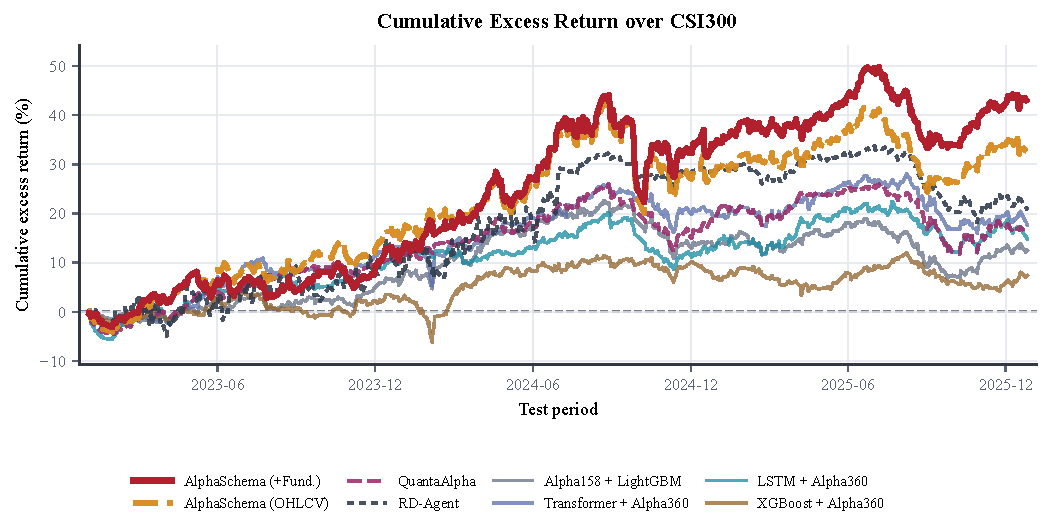
\includegraphics[width=\columnwidth]{figures/cumulative_Excess_Return.pdf}
    \caption{Held-out cumulative excess return against representative
    open-source factor libraries on CSI300 over the 2023--2025 test period. All
    curves are evaluated under the same CSRankNorm, LightGBM combiner, and
    Top50/Drop5 backtest protocol.}
    \label{fig:cumulative_excess_return}
\end{figure}

\subsection{Ablation Study}

We first test whether each semantic schema field is necessary. Unless otherwise noted, all variants share the same search budget, LLM backbone, downstream LightGBM combiner, and backtest protocol.




\subsubsection{Component Ablation of the Schema Grammar}

The second group targets the semantic grammar itself. We fix a set of 100 high-reward full schema plans and construct five blind leave-one-out variants for each plan, removing exactly one field from \{\emph{Event}, \emph{Context}, \emph{Qualities}, \emph{Direction}, \emph{Output}\}. The code agent observes only the remaining fields and is not told which field is missing. This design isolates the contribution of individual schema fields from differences in search trajectory: all variants originate from the same full-plan set, while degradation is measured after guarded implementation and factor evaluation. Since a single informative factor can be useful with either sign, we use mean absolute Rank IC as the primary diagnostic metric.

\begin{figure}[!t]
    \centering
    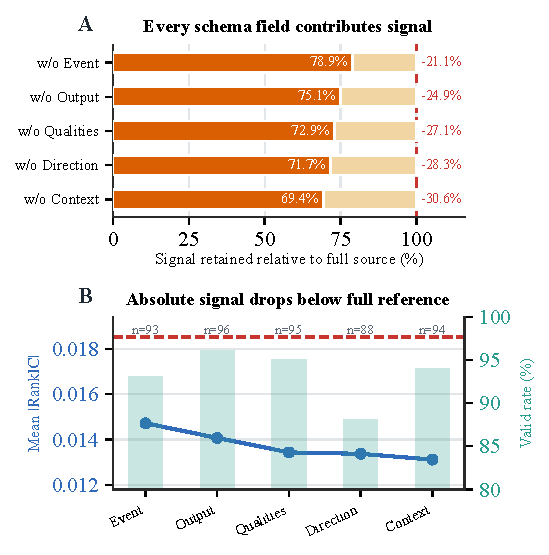
\includegraphics[width=\columnwidth]{figures/schema_component_ablation.pdf}
    \caption{Component-wise schema ablation.}
    \label{fig:schema_leave_one_out}
\end{figure}

Figure~\ref{fig:schema_leave_one_out} summarizes the leave-one-field-out results. Panel A reports retained signal strength relative to the full source reference, and Panel B separates mean \(|\mathrm{RankIC}|\) from implementation validity. All five removals reduce signal strength, retaining only 69.4\%--78.9\% of the full-plan reference. The largest degradation occurs when \emph{Context} is removed, suggesting that regime and reference conditioning are central to converting an economic event into a useful cross-sectional signal. The schema benefit is therefore distributed across fields rather than carried by a single descriptor.

\subsection{Backend Robustness Analysis}

We test whether schema-guided realization depends on a single implementation agent. Holding 100 schema plans fixed, six code-agent backends implement the same plans, with at most one retry for failed cases when available. Final success rates range from 82\% to 99\%, while mean \(|\mathrm{RankIC}|\) over successful implementations remains in a comparable range (0.0116--0.0168). Figure~\ref{fig:code_agent_model_invariance} separates these two effects: Panel A reports pass@1 success and repair recovery, and Panel B reports post-success signal quality. The result suggests that backend choice mainly affects execution reliability, while the semantic plan and the resulting factor function transfer across different code agents. Appendix~\ref{sec:appendix_code_agent_robustness} provides the full table.

\begin{figure}[!t]
    \centering
    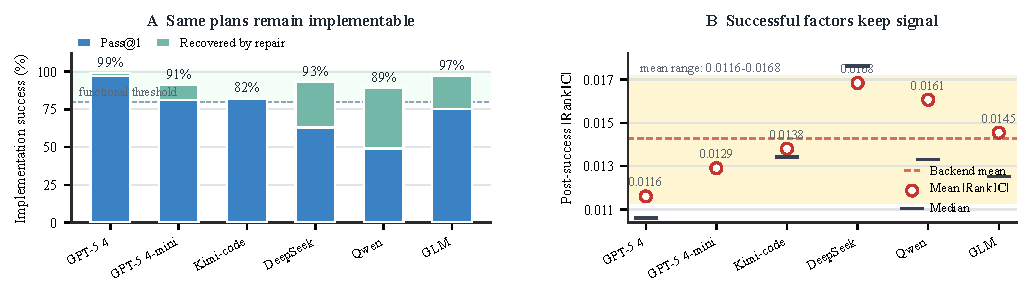
\includegraphics[width=\columnwidth]{figures/code_agent_model_invariance.pdf}
    \caption{Repair-aware robustness to code-agent backends on the same 100 schema plans. Panel A separates first-attempt implementation success from repair recovery; Panel B shows that successful implementations retain comparable signal quality across backends.}
    \label{fig:code_agent_model_invariance}
\end{figure}

\subsection{Schema-Space Predictability Analysis}

We further ask whether schema rewards are predictable before code realization. We collect 12,126 historical plan--reward pairs covering 11,295 unique schema keys and train lightweight predictors using only discrete schema features. \emph{Single schema} uses component-level indicators and category/scope counts, while \emph{Schema + pair} additionally includes pairwise component interactions. No schema text embeddings, generated code, factor values, or backtest trajectories are used as inputs.

\begin{figure}[!t]
    \centering
    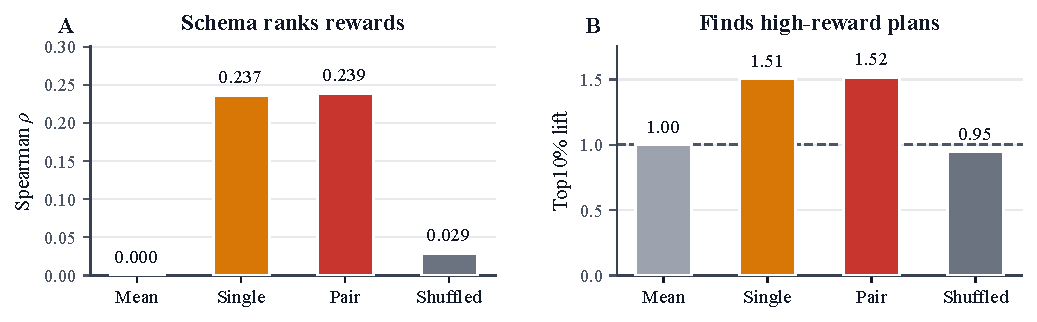
\includegraphics[width=\columnwidth]{figures/schema_space_predictability.pdf}
    \caption{Schema-space reward predictability.}
    \label{fig:schema_predictability}
\end{figure}

Figure~\ref{fig:schema_predictability} shows that schema-level features are predictive under this restricted setting. Panel A compares reward-ranking quality, while Panel B reports top-decile enrichment for the mean baseline, the single-schema LightGBM scorer, the pair-interaction LightGBM scorer, and the shuffled-reward control. Single-schema LightGBM reaches Spearman \(0.237\) and top-decile lift \(1.506\), while adding pair interactions improves the lift to \(1.519\). The mean baseline has no ranking ability, and the shuffled-reward control remains near random, indicating that the signal is tied to the true schema--reward association rather than model capacity alone.
